\documentclass[hidelinks,a4paper,12pt]{article}
\addtolength{\oddsidemargin}{-1.cm}
\addtolength{\textwidth}{2cm}
\addtolength{\topmargin}{-2cm}
\addtolength{\textheight}{3.5cm}
\newcommand{\HRule}{\rule{\linewidth}{0.5mm}}
\makeindex

\usepackage{longtable}
\usepackage[pdftex]{graphicx}
\usepackage{makeidx}
\usepackage{hyperref}
\hypersetup{
    colorlinks=true,
    linkcolor=blue,
    filecolor=magenta,      
    urlcolor=cyan,
}


% define the title
\author{Men-at-Work}
\title{ OnlyRugby Architectural Requirements}
\begin{document}
\setlength{\parskip}{6pt}

% generates the title
\begin{titlepage}

\begin{center}
% Upper part of the page       

\includegraphics[width=1\textwidth]{./up-logo.jpg}\\[0.4cm]    
\textsc{\LARGE Department of Computer Science}\\[1.5cm]
\textsc{\Large COS 301 - Software Engineering}\\[0.5cm]
% Title
\HRule \\[0.4cm]
{ \huge \bfseries OnlyRugby\\Architectural Requirements}\\[0.4cm]
\HRule \\[0.4cm]
% Author and supervisor
\begin{minipage}{0.4\textwidth}
\begin{flushleft} \large
\emph{Authors:}
\end{flushleft}
\end{minipage}
\begin{minipage}{0.4\textwidth}
\begin{flushright} \large
\emph{Student number:}
\end{flushright}
\end{minipage}

\begin{minipage}{0.4\textwidth}
\begin{flushleft} \large
Herman {Keuris}
\end{flushleft}
\end{minipage}
\begin{minipage}{0.4\textwidth}
\begin{flushright} \large
\emph{}
u13037618
\end{flushright}
\end{minipage}

\begin{minipage}{0.4\textwidth}
\begin{flushleft} \large
Johan {van Rooyen}
\end{flushleft}
\end{minipage}
\begin{minipage}{0.4\textwidth}
\begin{flushright} \large
\emph{}
u11205131
\end{flushright}
\end{minipage}

\begin{minipage}{0.4\textwidth}
\begin{flushleft} \large
Estian {Rosslee}
\end{flushleft}
\end{minipage}
\begin{minipage}{0.4\textwidth}
\begin{flushright} \large
\emph{}
u12223426
\end{flushright}
\end{minipage}

\begin{minipage}{0.4\textwidth}
\begin{flushleft} \large
Ivan {Henning}
\end{flushleft}
\end{minipage}
\begin{minipage}{0.4\textwidth}
\begin{flushright} \large
\emph{}
u13008219
\end{flushright}
\end{minipage}

\begin{minipage}{0.4\textwidth}
\begin{flushleft} \large
Muller {Potgieter}
\end{flushleft}
\end{minipage}
\begin{minipage}{0.4\textwidth}
\begin{flushright} \large
\emph{}
u12003672
\end{flushright}
\end{minipage}

\vfill
% Bottom of the page
{\large \today}
\end{center}
\end{titlepage}
\footnotesize
%\input{declaration_of_originality.tex}
\normalsize


\pagenumbering{roman}
\tableofcontents
\newpage
\pagenumbering{arabic}

\newpage
\section{Introduction} This section deals with the software architecture requirements of the OnlyRugby App. This includes:
	\begin{itemize} 
		\item The architectural scope.
		\item Quality requirements.
		\item The integration and access channel requirements.
		\item The architectural constraints.
		\item Architectural patterns and styles used.
		\item The architectural tactics and strategies used.
		\item The use of reference architectures and frameworks.
		\item Access and integration channels.
		\item Technologies used.
	\end{itemize}

\section{Architecture Requirements}
	\subsection{Architectural Scope}
	The following responsibilities need to be addressed by the software architecture:
	\begin{enumerate}
		\item To be able to host and provide an execution environment for the services/business logic of the system.
		\item To provide an infrastructure that provides a mobile access channel
		\item To provide an infrastructure that handles both local and remote persisting and provides access to domain objects.
		\item To integrate with the OnlyRugby social platform's MySQL database
	\end{enumerate}
\subsection{Quality Requirements}
	The following quality requirements are in order of the most important to least important (can be changed as the project progresses).	
	\subsubsection{Critical:}
	\subsubsection*{Usability}
	The average individual should be able to use the OnlyRugby app without any prior training and not be discouraged from using the system again.
	\begin{itemize}
		\item The OnlyRugby app's interface must be efficient, easy to use, and intuitive to navigate. To accomplish this the interface should be kept minimalistic and logical to allow the user to easily identify and use the services provided by the app.
		\item Initially only English needs to be supported, however the system must allow for translations to other internationally spoken languages (To allow for an increased user base once the system is made available for regions outside South Africa)
		\item Usability tests will involve typical users using the OnlyRugby app in a realistic (yet simulated) environment. Tests will be recorded on video as this medium provides task completion time and allows for observation of the user's behaviour, emotions, and difficulties while using the app.
	\end{itemize}
	
	\subsubsection*{Scalability}
	Since the system is planned to be made available for use internationally, it is vital to the success of the system that a large number of users can be accommodated.
	\begin{itemize}
		\item Management of resources available to the app across a range of Android devices needs to scale to ensure that every user of the OnlyRugby app will be presented with a satisfactory experience.
		\item The system must be able to operate effectively under the load of one user per team for all teams that are registered on the OnlyRugby social platform. (Ball park figure of ~1500 after complete deployment in South Africa, 1526 clubs registered with the Rugby Union of South Africa)
	\end{itemize}

	\subsubsection{Important:}

	\subsubsection*{Availability}
	Due to the live data capturing requirements of the application and the future planned international release it is important that the OnlyRugby system is always accessible to the user, at the very least during all rugby games registered on the OnlyRugby social platform.
	\begin{itemize}
		\item The OnlyRugby app must be accessible on the multitude of android devices running Android 4.0 and above.
		\item Data should be captured and stored locally before being pushed to the server in order to avoid data loss should the device being used lose connection to the server for any reason. This way even if the server is down the core functionality of the app is still usable.
	\end{itemize}

	\subsubsection*{Integrability}
	The system must be able to communicate with the OnlyRugby social platform.
	\begin{itemize}
		\item Must integrate with the social platform's database concerning teams, players, and scheduled games for retrieval of display information. If communication is not possible (e.g. a loss of data connection) then default/place-holder values (e.g. Team 1, Player number 23) should be used for local storage and replaced with actual data once the connection is restored, but before data is pushed to the server.
	\end{itemize}
	\subsubsection*{Maintainability}
	The OnlyRugby app system must be maintained to keep the system in a continual safe operating state.
	\begin{itemize}
		\item Should the system go down then it will be rolled back to a previous state in which the system was safe. This lets us recover from an error or a system fault.
		\item Corrective maintenance is implemented to correct discovered problems in the system after the system has broken. This is the most expensive form of maintenance.
		\item Preventative maintenance is implemented to correct discovered problems in the system after the system has been implemented but before the system breaks down.
	\end{itemize}
	
	\subsubsection*{Testability}
	All the different modules of the OnlyRugby app system must be tested thoroughly before they are integrated and deployed in the final system.
	\begin{itemize}
		\item Each service provided by the system must be testable through a unit test that tests:
		\begin{itemize}
			\item That the service is provided if all pre-conditions specified in the service contract are met.
			\item That all post-conditions specified in the service contract hold true once the service has been provided.
		\end{itemize}
	\end{itemize}
	
	\subsubsection*{Monitorability and Auditability}
	User activities should be logged so that they can be audited at a later stage. Each action on the system must be recorded in an audit log that can be viewed and queried at a later date should the necessity to do so arise.
	Information to be recorded must include:
	\begin{itemize}
		\item The identity of the individual carrying out the action.
		\item A summary description of the action.
		\item A timestamp indicating when action was performed.
	\end{itemize}
	
	Other information may be logged which may provide useful statistical information about the system while in use. Examples of such data to be logged might include:
	\begin{itemize}
		\item Location data.
		\item Failure to communicate with server.
		\item How long data was kept in local storage before being pushed to the server successfully.
		\item Miscellaneous errors.
	\end{itemize}
	
	\subsubsection{Nice to have:}
	
	\subsubsection*{Security}
	All system functionality is accessible to users who can be successfully authenticated against the user database. If connection to the server is not available functionality will be granted in a guest mode and the user will be asked to authenticate prior to the data being pushed to the server upon re-establishment of connection.
	\begin{itemize}
		\item All communication of sensitive data must be done securely through encryption and secure channels.
	\end{itemize}
	
	\subsubsection*{Performance requirements}	
	Long delays cause user frustration, may lead users to believe the system is not functioning, or that input has been ignored. To prevent this it is necessary to minimize the response time of user input to the system to ensure that the system works efficiently in real time.
	\begin{itemize}
		\item Performance will be measured with a scale of user frustration.
		\item Steps on the scale indicate how long a service takes to respond to the user.
		\item The three steps to be used are 0.1s, 1s, and 10s.
	\end{itemize}				

\subsection{Architectural Constraints}		
	The following architecture constraints have been imposed by the client:
		\begin{enumerate}
			\item The system must be developed using the following technologies
			\begin{itemize}
				\item Laravel PHP framework
				\item Google's Material Design
				\item Android 4.0+
				\item SQLite
			\end{itemize}
		\end{enumerate}

\section{Architecture Patterns or Styles}
	\subsection{Layered Architectural Strategy}
	The OnlyRugby application will make use of a 4-tier layered pattern, as explained below:
	\begin{enumerate}
		\item Presentation Layer:
		The Presentation Layer is comprised of two main aspects:
		\begin{enumerate}
			\item Interface: Provides an interface/front-end through which users/clients can access and interact with the Application Layer.
			\item Client Data Access: Captures the client's input and and passes it on to the Application Layer. Also responsible for validating input (but not for authentication).
		\end {enumerate}
		\item Application Layer:
		\begin{itemize}
			\item Provides back-end services of the system (i.e. all functions and forms of data processing/manipulation).
			\item Manages access to the web-services layer.
			\item Manages client login authentication.
			\item Manages persistence to the main database.
			\item If the app can not currently reach the database then this layer will provide a space to temporarily store all relevant data which needs to be uploaded to the database at a later time.
		\end {itemize}
		\item Web-services Layer:
		This layer is where the server is situated.
		\begin{itemize}
			\item Receives the processed client input from the Application Layer and adds it to the database (i.e. allows reading from- and writing to database).
			\item Provides other server-side computation/services such as:
				\begin{itemize}
					\item Conflict resolution when two different clients upload match statistics.
					\item Sending emails to clients (for example when registering with OnlyRugby).
				\end{itemize}
		\end{itemize}
		\item Data Layer:
		This layer is where the database is situated.
		\begin{itemize}
			\item Stores all added information, even when the client is not communicating with the database (i.e. persists data).
		\end{itemize}

		Reasons for choosing a layered architecture:
		\begin{itemize}
			\item Complexity is reduced by abstracting and separating a number of well defined layers which are then weakly coupled with each other. This allows the responsibilities of the system to be divided between the different layers and can prevent certain aspects of the system from becoming too dependant on (or needlessly intertwined with) another aspect of the system.
			\item It allows for the possibility of layers, at times, being re-used across the system (for example the Presentation Layer relies on the Application Layer to verify all input whereas the Web-services Layer relies on the Application Layer to format the input so that it could be stored in the database).
			\item Separating certain aspects (such as interface and implementation) makes it easier to separate test different parts of the system.
			\item The reduced dependency of various parts of the system on each other will also improve maintainability as it allows parts of the system to be updated without requiring any unnecessary changes to other parts of the system.
		\end{itemize}
		\begin{center}
  	 		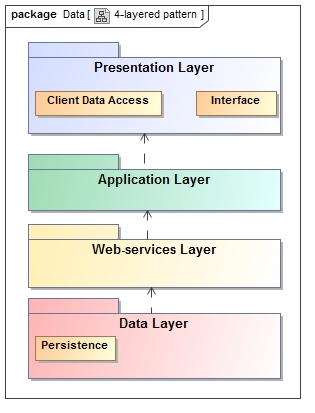
\includegraphics[width=0.5\textwidth] {./4-layered-pattern.jpg}\\[0.4cm]
		\end{center}
	\end{enumerate}
	
\section{Architectural strategies and tactics}
	\begin{enumerate}
	
		\item Authorization:
		The user’s profile on the application is authorized against the one on the database. JSON web tokens are passed between the application and the database. These tokens are very small, but can contain all the relevant data that needs to be passed and making use of these tokens makes it so that the database does not have to keep of sessions. These tokens are widely used, as they can be easily authorized and encrypted.

		The quality requirements addressed:
		\begin{itemize}
			\item Performance: Because the tokens are small, they will be easy and quick to process.
			\item Security: By encrypting the tokens and authorizing the user, private information can be protected.
			\item Auditability and Testability: Sending the indormation in these tokens will make it easier to see if the correct data was passed.
		\end{itemize}
		
		\item Queuing and scheduling:
		Queuing and scheduling can be used to maximize the performance of the application and the server. As new requests are received, they are placed into a queue and sequentially processed. This will assure fairness and that requests are processed in order. This will also be used if a user does not have internet access, but wishes to load new statistics. The data will be queued, until it can be sent.

		The quality requirements addressed:
		\begin{itemize}
			\item Availability, by optimizing the processing of the requests.
			\item Reliability and audit ability. This way, the order in which requests are processed can be guaranteed.
			\item Auditability and Testability: Sending the indormation in these tokens will make it easier to see if the correct data was passed.
		\end{itemize}
		
		\item Ping / Echo:
		Ping is a computer network administration software utility used to test the reachability of a host on an Internet Protocol (IP) network and to measure the round-trip time for messages sent from the originating host to a destination computer and back. By having the application send these pings on a regular basis, perhaps daily and when the user logs in, to the database, it can ensure that it still has access to the central server and that it is up to date with both the latest statistics, as well as the newest version of the application.

		The quality requirements addressed:
		\begin{itemize}
			\item Security. As it can ensure that all its security policies are up to date and that it can report any faults/errors.
			\item Availability. It will inform the user if it was unable to reach the server.
			\item Reliability. Any issues that arise may be reported and it ensures that a connection is available.
			\item Monitor-ability and Audibility. It can log faults detected.
			\item Testability. It will allow us to test the connection to the server and that it can make use of said connection.
		\end{itemize}
		
		\item Message integrity:
		We will be exchanging JSON files between the server and the application. These files will include any new data that either party may need. By including a checksum, these files can be checked for any errors that may have occurred during transportation. Should it find a checksum error, a request will be send and a new JSON file will be transmitted.

		The quality requirements addressed:
		\begin{itemize}
			\item Security. This will help to protect the system from corrupted data that may hamper the application and/or server's functionality.
			\item Reliability: This will help ensure that erroneous data is not used.
			\item Monitorability and Auditability: It will allow us to test if the application and/or server constantly sends erroneous data and address the issue.
		\end{itemize}
		
		\item Multi-Threading:
		By using multiple threads, the application can process a larger amount of data simultaneously. While the user may be busy updating a game's statistics, the application will assign another thread to process any incoming requests, improving the program's overall performance.

		The quality requirements addressed:
		\begin{itemize}
			\item Performance. It will be able to process more data, simultaneously.
			\item Flexibility. By creating new threads, the program will be able to handle multiple tasks more easily.
			\item Usability. By keeping the user unaware of any background actions that are taking place, it will be easier for them to use the app.
		\end{itemize}
	\end{enumerate}

\section{Use of reference architectures and frameworks}
	The reference architecture that will be used is Java Platform Enterprise Edition. This architecture was chosen because our system is based on a layered architecture. The framework that will be used is the Laravel PHP Framework as we will have a RESTful web service.

\section{Access and integration channels}
	\subsection{Human access channels}
	\begin{itemize}
		\item Must be able to access services through the OnlyRugby application installed on tablets and phones running Android 4.0+
		\item The user can easily use the OnlyRugby application to communicate with the server (when registering, logging on and off of their profiles) and through the server they can communicate with the MySQL database.
		\item Quality requirements addressed:
			\begin{itemize}
				\item Availability
				\item Usability
			\end{itemize}
	\end{itemize}

	\subsection{System access channels}
	The OnlyRugbyApp system can only be directly accessed through a web page (i.e. using http) using the REST API provided by the server. \\
	Quality requirements addressed:
	\begin{itemize}
		\item Security
	\end{itemize}

	\subsection{Integration Channel Used}
	\subsubsection {REST - Representational State Transfer}
	\begin{itemize}
		\item Uses standard HTTP and thus simpler to use.
		\item Allows different data formats where as SOAP only allows XML.
		\item Has JSON support (faster parsing than XML).
		\item Better performance and scalability with the ability to cache reads.
		\item Protocol Independent, can use any protocol which has a standardised Uniform Resource Identifier (URI) scheme.
		\item Quality requirements addressed:
			\begin{itemize}
				\item Integrability
				\item Maintainability
			\end{itemize}
	\end{itemize}

	\subsection{Protocols}
	\subsubsection {HTTP - Hypertext Transfer Protocol}
	\begin{itemize}
		\item Used to respond to requests and transfer data
	\end{itemize}
	\subsubsection {IP - Internet Protocol}
	\begin{itemize}
		\item Allows communications between client and server
		\item In charge of sending, receiving and addressing data packets.
	\end{itemize}
	\subsubsection {SMTP - Simple Mail Transfer Protocol}
	\begin{itemize}
		\item Used to send emails (useful for registration confirmation)
		\item MIME (Multi-purpose Internet Mail Extensions) which allows SMTP
to send multimedia files.
	\end{itemize}
	\subsubsection {TSL - Transport Layer Security}
	\begin{itemize}
		\item Alternative to SSL.
		\item Newer and more secure version of SSL.
	\end{itemize}		
		
\section{Technologies}
	\subsection{Programming technologies}
		\subsubsection{Android Studio}
			Android studio will be used as the IDE and the app will be backwards compatible from Android 4.0. 
		\subsubsection{MySql}
			MySql will be used for the web server database.
		\subsubsection{SQLite}
			SQLite will be used for the local on device database.
	\subsection{Web technologies}
		\subsubsection{RESTful web service}
			Laravel PHP framework will be used to create a RESTFul web api to interact with the web server database and provide data persistence
		
\end{document}
